\documentclass[border=10pt]{standalone}

\usepackage{tikz}
\usepackage{tikzsymbols}
\usetikzlibrary{calc,patterns,shapes.geometric}

\def\centerarc[#1](#2)(#3:#4:#5){\draw[#1] ($(#2)+({#5*cos(#3)},{#5*sin(#3)})$) arc (#3:#4:#5);}

\begin{document}
	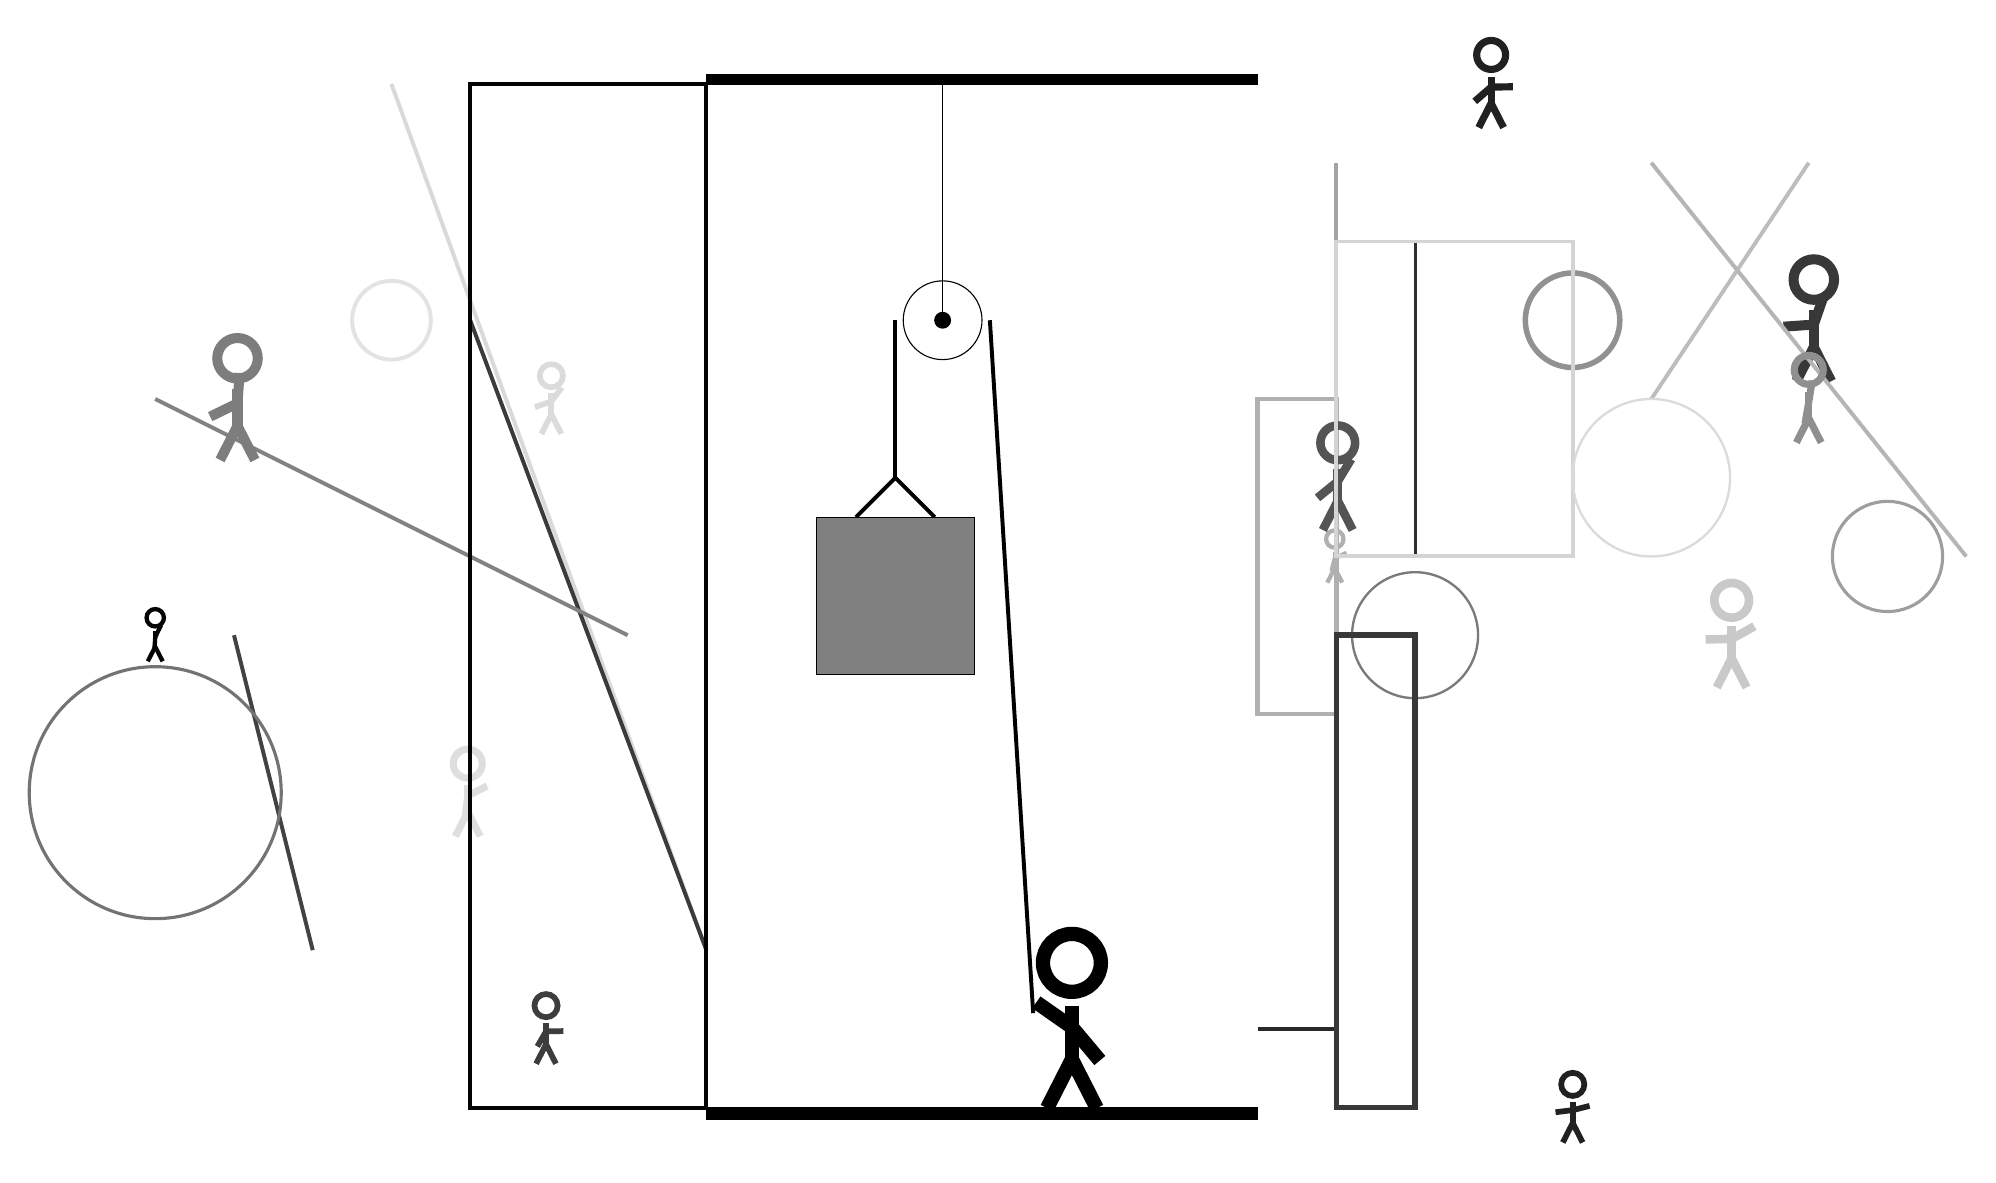
\begin{tikzpicture}
		%%%%% START %%%%%
		
		\draw[fill=black] (-2, 10) rectangle (5, 10.125);
		
		\draw (1, 7) circle (0.5);
		\draw[fill=black] (1, 7) circle (0.1);
		\draw (1, 10) -- (1, 7);
		
		\draw[line width=0.5mm] (-0.1, 4.5) -- (0.4, 5.0) -- (0.9, 4.5);
		\draw[fill=black!50] (-0.6, 4.5) rectangle (1.4, 2.5);
		
		\node[line width=0.4mm, color=black!78] at (12, 7) {\Strichmaxerl[7][4][71]};
		
		\draw[line width=0.5mm, color=black!15](-6, 10) -- (-2, -1);
		\draw[line width=0.4mm, color=black!82] (6, 4) rectangle (7, 8);
		\draw [line width=0.3mm, color=black!52](7, 3) circle (0.8);
		\node[line width=0.3mm, color=black!13] at (-5, 1) {\Strichmaxerl[5][83][27]};
		\draw [line width=0.5mm, color=black!11](-6, 7) circle (0.5);
		
		\draw[line width=0.6mm, color=black!31] (5, 6) rectangle (6, 2);
		\node[line width=0.2mm, color=black!98] at (-9, 3) {\Strichmaxerl[3][86][64]};
		\node[line width=0.6mm, color=black!31] at (6, 4) {\Strichmaxerl[3][76][25]};
		
		\draw[line width=0.5mm, color=black!26](10, 6) -- (12, 9);
		\draw[line width=0.5mm, color=black!36](6, 9) -- (6, 8);
		\node[line width=0.4mm, color=black!87] at (8, 10) {\Strichmaxerl[5][41][1]};
		\draw [line width=0.7mm, color=black!43](9, 7) circle (0.6);
		
		\draw [line width=0.4mm, color=black!38](13, 4) circle (0.7);
		\node[line width=0.5mm, color=black!76] at (-4, -2) {\Strichmaxerl[4][60][1]};
		\draw[line width=0.5mm, color=black!29](10, 9) -- (14, 4);
		
		\draw[line width=0.5mm, color=black!77](-5, 7) -- (-2, -1);
		\draw[line width=0.5mm, color=black!49](-3, 3) -- (-9, 6);
		\node[line width=0.4mm, color=black!51] at (-8, 6) {\Strichmaxerl[7][26][86]};
		\draw[line width=0.5mm, color=black!84](5, -2) -- (6, -2);
		\node[line width=0.2mm, color=black!14] at (-4, 6) {\Strichmaxerl[4][19][53]};
		\node[line width=0.3mm, color=black!44] at (12, 6) {\Strichmaxerl[5][80][81]};
		
		\node[line width=0.4mm, color=black!67] at (6, 5) {\Strichmaxerl[6][39][59]};
		\draw[line width=0.5mm, color=black!17] (6, 8) rectangle (9, 4);
		\node[line width=0.7mm, color=black!21] at (11, 3) {\Strichmaxerl[6][1][29]};
		
		\node[line width=0.5mm, color=black!87] at (9, -3) {\Strichmaxerl[4][7][14]};
		\draw[line width=0.7mm, color=black!78] (7, 3) rectangle (6, -3);
		\draw[line width=0.5mm, color=black!99] (-2, 10) rectangle (-5, -3);
		
		\draw[line width=0.5mm, color=black!74](-7, -1) -- (-8, 3);
		
		\draw [line width=0.4mm, color=black!55](-9, 1) circle (1.6);
		\draw [line width=0.3mm, color=black!14](10, 5) circle (1.0);
		
		\draw[line width=0.5mm] (0.4, 7) -- (0.4, 5.0);
		\centerarc[line width=0.5mm](1, 7)(0:180:0.6);
		\draw[line width=0.5mm](1.6, 7) -- (2.15, -1.8);
		
		\node at (2.6, -1.9) {\Strichmaxerl[10][-35][-50]};
		
		\draw[fill=black] (-2, -3) rectangle (5, -3.15);
		
		%%%%% END %%%%%
	\end{tikzpicture}
\end{document}